% arara: xelatex: { shell: yes }
% arara: makeglossaries
% arara: biber
% arara: xelatex: { shell: yes }
% arara: xelatex: { shell: yes }

\documentclass[thesis=B,czech]{template/FITthesis}[2019/03/06]
\selectlanguage{czech}

\usepackage[style=iso-numeric]{biblatex}
\usepackage[utf8]{inputenc}

\usepackage{dirtree}
\usepackage{minted, xcolor}
\usemintedstyle{friendly}
% \definecolor{bg}{HTML}{282828}
% \setminted{bgcolor=bg}

\usepackage{csquotes}
\usepackage{xevlna}
\usepackage{pgfplots}

\bibliography{bybliography}


% % list of acronyms
\usepackage[acronym,nonumberlist,toc,numberedsection=autolabel]{glossaries}
\iflanguage{czech}{\renewcommand*{\acronymname}{Seznam pou{\v z}it{\' y}ch zkratek}}{}
\makeglossaries

\newcommand{\tg}{\mathop{\mathrm{tg}}} %cesky tangens
\newcommand{\cotg}{\mathop{\mathrm{cotg}}} %cesky cotangens

\department{Katedra softwarového inženýrství}
\title{Specializovaná webová aplikace pro výuku hry na ukulele}
\authorGN{Dan} %(křestní) jméno (jména) autora
\authorFN{Balarin} %příjmení autora
\authorWithDegrees{Dan Balarin} %jméno autora včetně současných akademických titulů
\author{Dan Balarin} %jméno autora bez akademických titulů
\supervisor{Ing. Marek Suchánek}
\acknowledgements{TODO\: Doplňte, máte-li komu a za co děkovat. V~opačném případě úplně odstraňte tento příkaz.}
\abstractCS{Bakalářská práce se zabývá vývojem webové aplikace podporující výuku hraní na ukulele. Aplikace je vyvíjena v~souladu s~metodami softwarového inženýrství. Zkoumá existující řešení, dostupné technologie a cílovou skupinu. Následně stanoví formalní požadavky na aplikaci a dané požadavky implementuje a testuje. V~poslední části rozebírá automatické testování a nasazování.}
\abstractEN{Bachelor thesis decsribes the development of web application for learning how to play on the ukulele. The application is developed according to methods of software engineering. Thesis researches existing solutions, available technologies, and target audience. After that, it sets formal requirements on application and implements and tests these requirements. The last part is focused on automatic testing and deployment.}
\placeForDeclarationOfAuthenticity{V~Praze}
\declarationOfAuthenticityOption{4} %volba Prohlášení (číslo 1-6)
\keywordsCS{ukulele, metronom, akordy, interaktivní výuka, webová aplikace, React, GraphQL, kontinuální integrace, automatické nasazování}
\keywordsEN{ukulele, metronome, chords, interactive lessons, web application, React, GraphQL, continuous integration, automatic deployment}
\website{https://github.com/danbalarin/bachelors-thesis} %volitelná URL práce, objeví se v tiráži - úplně odstraňte, nemáte-li URL práce

\newglossaryentry{strumming pattern}
{
        name={strumming pattern},
        description={Způsob brnkání na struny}
}

\newglossaryentry{tree shaking}
{
        name={tree shaking},
        description={Odstranění nepoužité části knihovny}
}


\newacronym{npm}{npm}{Node Package Manager}
\newacronym{pnp}{PnP}{Plug'n Play}
\newacronym{nra}{NRA}{Node Resolution Algorithm}
\newacronym{api}{API}{Application Programming Interface}
\newacronym{seo}{SEO}{Search Engine Optimalization}
\newacronym{rest}{REST}{Representational state transfer}
\newacronym{ssr}{SSR}{Server Side Rendering}
\newacronym{orm}{ORM}{Object Reloation Mapping}


\newcommand{\smallindentsize}{1cm}

\newenvironment{usecase}[2]{
    \noindent
    \paragraph{#1}
    \label{#2}
    \begin{smallindent}{}
        }{
    \end{smallindent}
}

\newenvironment{scenario}[2]{
    \paragraph{#1}
    \label{#2}
    \begin{enumerate}
        }{
    \end{enumerate}
}

\newenvironment{requirment}[2]{
    \noindent \begin{minipage}{\textwidth}
        \paragraph{#1}
        \label{#2}
        \begin{smallindent}{}
            }{
        \end{smallindent}
    \end{minipage}
}

\newenvironment{smallindent}{%
    \begin{adjustwidth}{\smallindentsize}%
        }{%
    \end{adjustwidth}%
    \bigskip
}


\graphicspath{{./assets/use_case_mode.png}}

\begin{document}

\begin{introduction}
    \label{ch:introduction}
    \section{Motivace}
    V posledních letech roste popularita hry na hudební nástroje a s rozvojem informačních technologií s tím souvisí i snaha uživatelů učit se sami za pomoci veřejně dostupných aplikací. Pro začátečníky se doporučují nástroje buď drnkací (ukulele, kytara) nebo dechové (harmonika, flétna)~\cite{s_2016_the}~\cite{richardson_2019_top}.

    Ukulele oproti kytaře má tu výhodu, že je menší, má o dvě struny méně, struny tolik neřežou do prstů a je tedy jednodušší pro začátečníka. Oproti nástrojům dechovým má hlavně tu výhodu, že se na něj dá zahrát více populárních písní.

    Aktuálně existuje již několik aplikací, ať už webových nebo mobilních, které umožňují uživateli učit se hrát na ukulele sám doma. Problémy těchto aplikací jsou, že jsou buď placené, neobsahují všechny funkcionality, nebo nejsou uživatelsky přívětivé. Rozborem již existujicích řešení se podrobněji zabývá kapitola \nameref{ch:analysis}.

    K této problematice jsem se dostal, jelikož jsem se sám začal učit hrát na ukulele. Již existujicí aplikace mi nevyhovují a to převážně kvůli chybějícím funkcím, nebo neintuitivnímu ovládání. Z tohoto důvodu mi přišlo ideální vytvořit vlastní aplikaci, která bude obsahovat veškeré funkce, chybějící u již existujících aplikací, bude snadno ovladatelná a bude fungovat na počítači i chytrém telefonu.


    \section{Cíle práce}
    Hlavním cílem práce je navrhout, vytvořit a otestovat aplikaci, která umožní začátečníkovi naučit se hrát na ukulele, čehož lze dosáhnout několika způsoby, kterými se budeme zabývat v kapitole \nameref{ch:analysis}. Dílčím cílem je umožnit již zkušenému hráči vyhledat jednotlivé akordy nebo akordy a text k písni.

    Důležitou součástí aplikace je jednoduchost použití, uživatelská přívětivost a zároveň možnost použití některých složitějších mechanismů, jako je například výuka přechytávání akordů s možností zapnutí metronomu, nebo vyhledávání v několika různých množinách (např. akordy, písně a autoři).

    \section{Členění práce}
    Práce je členěna do kapitol odpovídajících krokům vývoje software podle principů metodologie unifikovaného vývoje~\cite[s.~51‑68]{arlow_2007_uml}.

    Kapitola \nameref{ch:analysis} se zabývá průzkumem již existujících aplikací, zjištění cílové skupiny, dostupných technologií a platforem a možnostmi, jak k danému problému přistoupit.

    \hyperref[ch:design]{Druhá kapitola práce}, se věnuje návrhu aplikace. Návrh aplikace je nedílnou součástí vývoje složitějších systémů a aplikací. Umožní programátorovi, nebo týmu programátorů, mít lepší představu o celém projektu, zjistit nedostatky ještě před implementací, nebo například stanovit místa v aplikaci kde může v budoucnu dojít k rozšíření a aplikaci na to řádně připravit. Tato kapitola obsahuje formální stanovení požadavků na aplikaci a vytvoření náhledů uživatelského rozhraní.

    Kapitola \nameref{ch:implementation} rozebírá prostředí v jakém probíhal vývoj aplikace, konečný výběr technologií, určení logického členění a architektury aplikace a některé aspekty zdrojového kódu samotné aplikace. Správně zvolená architektura aplikace usnadní vývoj teď i případné rozšiřování, a může umožnit přepoužití části aplikace při práci na aplikaci jiné.

    \hyperref[ch:testing]{Čtvrtá kapitola} se věnuje testovaním aplikace. Testování je naprosto nezbytné pro vývoj kvalitní aplikace. Vývojář díky tomu zjistí, jakými nedostatky aplikace trpí ještě před tím, než na ně narazí uživatel. Jelikož tyto nedostatky mohou být kritické, může díky nim docházet k úniku citlivých informací a tím poškodit uživatele. Proto se každý systém a aplikace testuje a to na několika úrovních.

    \hyperref[ch:ci_cd]{Poslední kapitola} probírá automatické testování a nasazování. Automatizace testů a nasazování zrychluje vývoj a celkovou workflow týmu. Tato automatizace deleguje spouštění testů a buildů aplikace na dedikovaný server, takže se vývojář může zatím věnovat něčemu jinému.
\end{introduction}

\chapter{Analýza}
\label{ch:analysis}
Proces vývoje aplikace začíná u~analýzy. V~rámci analýzy se zkoumá daná problematika, kterou má aplikace řešit, již existující řešení, cílová skupina a možnosti řešení. Tato část je důležitá hlavně z~toho důvodu, abychom náhodou neřešili problém, který už někdo vyřešil za nás, nebo nevytvářeli aplikaci pro jinou cílovou skupinu, než bychom měli.

\section{Hra na ukulele}
\label{sc:ukulele_playing}
Jak již bylo zmíněno, ukulele je čtyřstrunný hudební nástroj, vzhledem podobný malé kytaře. Ukulele původně pochází z Havajských ostrovů, vzniklo z nástroje zvaného Braguinha a o původu jeho jména se vedou spekulace~\cite{rek_2008_kola}.

Samotné hraní je velmi podobné hře na kytaru, ukazováček, prostředníček, prsteníček a malíček levé ruky přitiskávají struny směrem k hmatníku, čímž určují akord a prsty pravé ruky přejíždějí po strunách někde na pomezí krku a těla ukulele. Způsobů jak držet akordy je několik a většinou záleží na dalším, resp. předchozím akordu, aby si hráč zjednodušil přechod. Stejně tak je i více způsobů jak přejíždět prsty po strunách. Prsty mohou jet dolů, nebo nahoru a to břískem nebo nehtem prstu, či lehce klepnout do těla a tím zároveň utlumit struny. Různým kombinacím těchto pohybů se říká \gls{strumming pattern}.

\subsection{Typy ukulele}
\label{ss:ukulele_types}
Ukulele má několik variant, které se odlišují velikostí nástroje a barvou zvuku.

Nejběžnější a zároveň doporučované pro začátečníky je ukulele sopránové. Sopránové ukulele je zároveň nejmenší a jeho běžné ladění je \textit{g,c,e,a} nebo \textit{a,d,f\textsuperscript{\#},h}.

Další ukulele jsou koncertní a tenorové, které jsou větší, ale ladí se stejně jako ukulele sopránové. Rozdíl je tedy v barvě zvuku a velikosti, tedy pohodlnosti držení.

Největší ukulele je barynotové, které je běžně laděné stejně jako vrchní čtyři struny kytary, tedy \textit{d,g,h,e}, a je vhodné pro hráče kteří již umí hrát na kytaru, právě kvůli stejnému ladění.

Další, méně obvyklé verze ukulele jsou šestistrunné, osmistrunné, desetistrunné a uke-benžo (benžolele), které vzniklo spojením ukulele a benža.


\section{Existující aplikace}
\label{sc:existing_apps}

\section{Dostupné technologie}
\label{sc:available_technologies}
Aplikace by měla být co nejdostupnější pro běžného uživatele, ideálně by tecy neměla vyžadovat stahování nebo instalaci. Z podstaty této aplikace to ani není potřeba. Jediná výhoda kterou přináší desktopová aplikace je přímý přístup k hardware a lepší výkon, jelikož ale tento typ aplikace nepotřebuje vykreslovat pokročilou 3D grafiku nebo spouštět složité algoritmy, tak je zbytečné se tím zabývat.

Nabízí se tedy webová aplikace nebo mobilní aplikace. Oba typy aplikací se dělí na dvě části, část kterou vidí a se kterou intereaguje uživatel nebo správce, která se nazývá frontend a část která obsluhuje práci s databází, zpracovává požadavky na změny, autorizuje uživatele, atd. Jeden backend přitom může obsluhovat frontend jak podobě webové, tak i mobilní aplikace. Rozdělíme si tedy sekce na \nameref{ss:backend}, \nameref{ss:web} a \nameref{ss:mobile}.

\subsection{Backend}
\label{ss:backend}
Backend tvoří páteř aplikací, zprostředkovává přístup k informacím, umožňuje úpravy a autorizuje uživatele. Z toho důvodu, je třeba dbát na kvalitu a hlavně bezpečnost kódu. Špatně autorizovaný uživatel, nebo nezabezpečená část databáze je velká bezpečnostní díra a tomu se musí předejít. Nedá se spoléhat na to, že uživatele ověřil frontend, jelikož se s daty na frontendu dá manipulovat (jak na webu, tak i v mobilu), a proto veškeré ověřování probíhá na serveru. Ověřování na frontendu tedy slouží jako čistě estetická záležitost.

Dalším důležitým faktorem je rychlost. Rychlost může ovlivnit několik faktorů, jako je třeba využití složitých algoritmů bez paralelizace, pomalý databázový server, nebo neoptimalizované databázové požadavky.

Při výběru je třeba tedy dbát hlavně na bezpečnost a rychlost. Avšak je třeba zvážit i tzv. code reuse, tedy částečné přepoužití kódu, které muže zjednodušit a zpřehlednit kód aplikace.

\subsubsection{Javascript}
Javascript je \textit{otevřený multiplatformní skriptovací jazyk pro tvorbu a přizpůsobení aplikací v podnikových sítích a na internetu.} \cite{netscapecommunicationscorporation_1995_press}, jako první implementovaný prohlížečem Netscape Navigator 2.0 a rychle adaptován ostatními prohlížeči.

Výhodou je multiplatformnost a jednoduchost vývoje a nasazení. Hlavní nevýhodou Javascriptu je, že Javascript je dynamicky typovaný, což vede k horší udržitelnosti kódu a odhalení většiny chyb až při běhu aplikace (absence statické kontroly). Tyto neduhy se dají odstranit použitím nějakou syntaktickou nadstavbou, jako je třeba Typescript nebo Flow, které přidávají statické typování proměnných a statickou kontrolu při překladu do Javascriptu.

Javascript se původně vyskytoval jen v prohlížeči, což znamená že nebyl použitelný pro vývoj desktopových a serverových aplikací. To se změnilo s příchodem Node.js. Node.js je prostředí, které umožňuje spouštět javascriptové skripty mimo prohlížeč.

\subsubsection{Java}
Staticky typovaný, multiplatformní programovací jazyk vycházející z jazyka C, zaštítěný firmou Oracle, Java, patří mezi nejpopulárnější a nejužívanější programovací jazyky \cite{stackexchangeinc_2019_stack} . Jeho hlavní užití je právě na straně serveru, a to v kombinaci s frameworkem Spring Boot \cite{jetbrainssro_2019_demographics} .

\subsubsection{C\# }
Jazyk velmi podobný Javě, vyvýjený firmou Microsoft. Jeho hlavní nevýhodou byla vysoká závislost na frameworku .NET, který až do příchodu alternativy .NET Core, byl spustitelný pouze na operačním systému Microsoft Windows.

\subsection{Web}
\label{ss:web}
Webová aplikace je pro uživatele nejpřístupnější formou, nemusí nic instalovat, stahovat, pouze otevře prohlížeč s webovou adresou a aplikaci má přístupnou a to jak na počítači, tak i na mobilu. Nevýhoda oproti mobilní aplikace je, že vyžaduje přístup k internetu (ne vždy, viz PWA **TODO**).

\subsubsection{Javascript}
Pro vývoj webové aplikace lze v Javascriptu zvolit z mnoha možností, ať už co se týče syntaktické nadstavby (Typescript, Flow), nebo knihoven a frameworků. Jelikož jich je velké množství, tak si jen stručně probereme tři nejpopulárnější a to React.JS, Angular a Vue.

React.JS je knihovna vyvýjená společností Facebook, která ho sama využívá pro tvorbu jejich aplikací jako je třeba Instagram, nebo WhatsApp. Jeho hlavní výhodou je možnost si spoustu věcí přizpůsobit k vlastní potřebě (např. routing, globalní uložiště dat, ...), což mimo jiné vede k menší velikosti výsledné aplikace a vyšší rychlosti. React sám o sobě není ani závislý na prohlížeči a může být využit např. pro vývoj aplikace spouštěné z příkazové řádky.

Angular je framework od společnosti Google, taktéž využívaný v řadě aplikací. Hlavní výhodou je, že Angular nabízí téměř vše co může programátor potřebovat, díky čemuž nemusí programátor řešit občasné potíže s kompatibilitou knihoven jako u Reactu, ale na druhou stranu je výsledná aplikace velká a pomalejší, jelikož obsahuje i nevyužívané funkce.

Vue je knihovna velmi podobná Reactu, sdílí spolu velkou část přístupů, ale Vue se zaměřuje na projekty malé až střední a React in na ty velké. Výhoda tedy je rychlost a jednoduchost, nevýhoda je, že ve velkém projektu se programátor, nebo tým programátorů může rychle začít ztrácet a zpomalí se vývoj.

\subsubsection{C\# }
V C\# se dá vyvýjet i frontend a to za pomoci frameworku ASP.NET, který závisí na frameworku .NET. V dnešní době se na nové projekty již příliž nevyužívá. Lze jej využít v kombinaci s Javascriptem a jeho knihovnami. Největší výhoda tohoto přístupu je striktní dodržení přístupu Model-View-Controler, nevýhodou jsou vyšší nároky na znalost obou technologií, což pro juniorního programátora může být problém.

\subsection{Mobil}
\label{ss:mobile}

\section{Cílová skupina}
\label{sc:target_audience}
Do cílové skupiny této práce se řadí kdokoliv kdo má zájem se naučit hrát na ukulele, celosvětově. To znamená, že uživatelem může být muž či žena od šesti do šedesáti let. Z toho se odvíjí požadavky na jazyk aplikace a uživatelskou přívětivost. Jelikož spektrum uživatelů je velmi rozsáhlé, tak uživatelské prostředí musí být jednoduché a přehledné. Webová aplikace umožní uživateli si aplikaci zobrazit jak na počítači, tak na mobilu či tabletu a zároveň nemá potřebu nic instalovat. Výchozím jazykem bude angličtina, protože je celosvětově rozšířenejší než čeština, ale aplikace musí být do budoucna připřavena mít více jazyků.



\chapter{Návrh}
\label{ch:design}

\section{Funkční požadavky}
\label{sc:functional_req}

\begin{requirment}{FP01 Metronom}{FP01}
    Aplikace zobrazí uživateli metronom. Uživatel má možnost zapnout či vypnout metronom a zvolit si rychlost.
\end{requirment}

\begin{requirment}{FP02 Akordy}{FP02}
    Aplikace umožní uživateli si zobrazit libovolnou podmnožinu akordů.
\end{requirment}

\begin{requirment}{FP03 Strumming pattern}{FP03}
    Aplikace zobrazí uživateli strumming pattern a metronom. Uživatel může ovládat metronom dle \hyperref[FP01]{FP01} a zobrazení strumming patternu reaguje na nastavení rychlosti metronomu.
\end{requirment}

\begin{requirment}{FP04 Vyhledávání}{FP04}
    Aplikace umožní uživateli vyhledávat písně, akordy a strumming patterny.
\end{requirment}

\begin{requirment}{FP05 Přechytávání akordů}{FP05}
    Aplikace umožní uživateli si vytvořit vlastní seznam akordů s volbou nastavení metronomu dle \hyperref[FP01]{FP01} a akordů dle \hyperref[FP02]{FP02}.
    Přihlášený uživatel má možnost si dané nastavení uložit pod libovolným jménem.
\end{requirment}

\begin{requirment}{FP06 Přechytávání akordů dle písně}{FP06}
    Aplikace zobrazí uživateli přechytávání akordů dle \hyperref[FP05]{FP05} s přednastavenými parametry podle vybrané písně.
\end{requirment}

\begin{requirment}{FP07 Zobrazení písně}{FP07}
    Aplikace zobrazí uživateli text písně, akordy písně a strumming pattern dle \hyperref[FP03]{FP03}. Uživatel má možnost přechodu na přechytávání akordů dle \hyperref[FP06]{FP06} a případně odkaz na přehrání písně na serveru třetí strany (např. youtube, spotify).
\end{requirment}

\begin{requirment}{FP08 Registrace}{FP08}
    Aplikace umožní zaregistrovat nového uživatele.
\end{requirment}

\begin{requirment}{FP09 Přihlášení}{FP09}
    Aplikace umožní uživateli se přihlásit.
\end{requirment}

\begin{requirment}{FP22 Odhlášení}{FP22}
    Aplikace umožní odhlásit přihlášeného uživatele.
\end{requirment}

\begin{requirment}{FP23 Úprava profilu}{FP23}
    Aplikace umožní přihlášenému uživateli měnit svoje údaje.
\end{requirment}

% \noindent \begin{minipage}{\textwidth}
%     \paragraph{FP13 Nastavení ladění} \label{FP13}
%     \begin{smallindent}{}
%         Aplikace nastaví ladění ukulele přihlášeného uživatele podle vstupu od uživatele.
%     \end{smallindent}
% \end{minipage}

\begin{requirment}{FP24 Označení písně jako oblíbená}{FP24}
    Aplikace umožní příhlášenému uživateli označit píseň jako oblíbenou.
\end{requirment}

\begin{requirment}{FP41 Vytvoření písně}{FP41}
    Aplikace umožňuje moderátorovi vytvořit nový záznam o písni.
\end{requirment}

\begin{requirment}{FP42 Úprava písně}{FP42}
    Aplikace umožňuje moderátorovi upravit existující záznam o písni.
\end{requirment}

\begin{requirment}{FP61 Úprava rolí uživatele}{FP61}
    Aplikace umožňuje administrátorovi změnit role uživatele.
\end{requirment}


\section{Nefunkční požadavky}
\label{sc:non_func_req}

\begin{requirment}{NP01 Kompatibilita}{NP01}
    Aplikace je dostupná přes webové rozhraní. Webové rozhraní poskytuje podporu pro prohlížeče Mozilla Firefox od verze 68, Google Chrome od verze 79 a Safari od verze 12.
\end{requirment}

\begin{requirment}{NP02 Podpora menších obrazovek}{NP02}
    Aplikace je responzivní, tedy se adaptuje na velikost obrazovky uživatele a podporuje dané prohlížeče na mobilních telefonech.
\end{requirment}

\begin{requirment}{NP03 SEO}{NP03}
    Aplikace je SEO-friendly, tedy splňuje všechny náležitosti pro internetové vyhledávače jako jsou Google nebo Seznam. Tyto náležitosti jsou testovány pomocí nástroje Google Lighthouse \cite{googlellc_2019_lighthouse}, kde aplikace musí dosáhnout celkového bodového ohodnocení alespoň 90 ze 100.
\end{requirment}

\begin{requirment}{NP04 API}{NP04}
    Aplikace vystavuje soukromé API a to ve formátu GraphQL.
\end{requirment}

\begin{requirment}{NP05 Rozšiřitelnost}{NP05}
    Aplikace je díky správnému návrhu a plánování možností rozšíření lehce rozšiřitelná.
\end{requirment}

\begin{requirment}{NP06 Lokalizace}{NP06}
    Aplikace je dostupná v anglickém jazyce.
\end{requirment}



\section{Uživatelské role}
\label{sc:user_roles}

\noindent \begin{minipage}{\textwidth}
    \paragraph{Uživatel}
    \begin{smallindent}{}
        Běžný uživatel, který se chce naučit hrát na ukulele nebo využít jinou funkcionalitu aplikace. Může použít metronom, učit se akordy, jejich přechytávání a nebo celou písničku.
        Má možnost se registrovat.
    \end{smallindent}
\end{minipage}


\noindent \begin{minipage}{\textwidth}
    \paragraph{Přihlášený uživatel}
    \begin{smallindent}{}
        To samé jako uživatel s možností se přihlásit, ukládat oblíbené písničky, vlastní přechytávání akordů. Dále má možnost si nastavit ladění vlastního ukulele, na což aplikace reaguje tak, že všude kde budou zobrazeny akordy, jmenovitě FP-002, FP-004-1, FP-004-2, tak má možnost přepnout mezi vlastním nastavením a výchozím.
    \end{smallindent}
\end{minipage}

\noindent \begin{minipage}{\textwidth}
    \paragraph{Moderátor}
    \begin{smallindent}{}
        To samé jako přihlášený uživatel s možností editovat písničky (akordy, strumming pattern, odkaz na ukázku).
    \end{smallindent}
\end{minipage}

\noindent \begin{minipage}{\textwidth}
    \paragraph{Administrátor}
    \begin{smallindent}{}
        To samé jako moderátor s možností upravovat role uživatelů.
    \end{smallindent}
\end{minipage}

\section{Případy užití}
\label{sc:use_cases}

\begin{usecase}{PU01 Metronom}{uc01}
    Případ užití umožňuje uživateli nastavovat parametry metronomu a ovládat ho. Mezi parametry patří tempo a způsob ukazování tempa (zvuková signalizace, blikání, odpočet, nebo vybrace na telefonu).

    \begin{scenario}{HS: Zobrazení metronomu}{uc01:hs}
        \item Scénář začne když uživatel zobrazí tuto komponentu.
        \item Aplikace zobrazí metronom a k~němu příslušející nastavení
    \end{scenario}

    \begin{scenario}{AS01: Zapnutí metronomu}{uc01:as01}
        \item Scénař začne když uživatel klikne na tlačítko \enquote{Start}
        \item Aplikace spustí metronom s~nastavenými parametry.
        \begin{itemize}
            \item Aplikace reaguje na změny parametrů okamžitě.
        \end{itemize}
        \item Tlačítko \enquote{Start} se změní na tlačítko \enquote{Stop} a scénář končí.
    \end{scenario}

    \begin{scenario}{AS02: Vypnutí metronomu}{uc01:as02}
        \item Scénař začne když uživatel klikne na tlačítko \enquote{Stop}
        \item Aplikace vypne metronom.
        \item Tlačítko \enquote{Stop} se změní na tlačítko \enquote{Start} a scénář končí.
    \end{scenario}
\end{usecase}

\begin{usecase}{PU02 Výuka akordů}{uc02}
    Případ užití umožní uživateli vyhledávat akordy a vybírat zobrazenou podmnožinu.
    % , přepínat mezi přednastavenými laděními ukulele (sopránové, barytonové) nebo si nastavit svoje vlastní. Pokud je uživatel přihlášen, pak má možnost si toto nastavení uložit jako svoje výchozí.

    \begin{scenario}{HS: Zobrazení akordů}{uc02:hs}
        \item Scénář začne po přechodu na stránku s~akordy.
        \item Aplikace zobrazí uživateli vyhledávací pole, které se řídí dle~\hyperref[uc02:as01]{AS01}
        % \item Aplikace zobrazí uživateli komponentu nastavování ladění, která se řídí dle~\hyperref[uc02:as02]{AS02}
    \end{scenario}

    \begin{scenario}{AS01: Vyhledání akordu}{uc02:as01}
        \item Scénář začne, když uživatel klikne do vyhledávacího pole nebo vyhledávací pole získá focus.
        \item Aplikace reaguje na vstup uživatele tak, že po každé změně hodnoty vyfiltruje akordy podle~\nameref{uc02:alg1}.
    \end{scenario}

    \begin{scenario}{AS02: Přechytávání akordů}{uc02:as02}
        \item Scénář začne, když uživatel vybere více než jeden akord.
        \item Aplikace umožní vybrané akordy řadit.
        \item Aplikace zobrazí uživateli komponentu z~\hyperref[uc01]{PU01}.
    \end{scenario}

    \begin{scenario}{AS03: Přechytávání akordů podle písně}{uc02:as03}
        \item Scénář začne při přechodu ze stránky písně.
        \item Aplikace nastaví hodnoty podle vstupu z~odkazu.
        \item Aplikace pokračuje~\hyperref[uc02:as02]{AS02}.
    \end{scenario}

    % \begin{scenario}{AS02: Přepnutí ladění podle přednastavené hodnoty}{uc02:as02}
    %     \item Scénář začne po výběru z nabídky přednastavených hodnot.
    %     \item Aplikace nastaví toto ladění jako aktualní ladění a scénář končí.        
    % \end{scenario}

    \begin{scenario}{Alg.1}{uc02:alg1}
        \item Pokud text začíná znakem z~množiny [\enquote{a}, \enquote{b}, \enquote{c}, \enquote{d}, \enquote{e}, \enquote{f}, \enquote{g}] pak filtruje výsledky podle daného znaku.
        \item Pokud text obsahuje podřetězec \enquote{maj}, pak vrátí pouze Major akordy.
        \item Pokud text obsahuje podřetězec \enquote{min}, pak vrátí pouze Minor akordy.
        \item Pokud text obsahuje jeden z~podřetězců [\enquote{dom}, \enquote{7}], pak vrátí pouze Dominant akordy.
        \item Vrátí vyfiltrované výsledky.
    \end{scenario}
\end{usecase}

\begin{usecase}{PU03 Výuka strumming patternů}{uc03}
    Případ užití umožní uživateli zobrazit stránku s výukou strumming patternů.

    \begin{scenario}{HS: Zobrazení výuky strumming patternů}{uc03:hs}
        \item Scénář začne po přechodu na stránku s výukou strumming patternů.
        \item Aplikace zobrazí uživateli stránku s výukou strumming patternů.
        \item Aplikace zobrazí uživateli komponentu z \hyperref[uc01]{PU01}.
        \begin{itemize}
            \item Pokud dojde k zapnutí/vypnutí metronomu, pak se spouští \hyperref[uc3:as02]{AS02}
        \end{itemize}
        \item Aplikace zobrazí uživateli komponentu z \hyperref[uc02]{PU02}.
    \end{scenario}


    \begin{scenario}{AS01: Výběr strumming patternu}{uc03:as01}
        \item Scénář začne když uživatel klikne na dropdown seznamu strumming patternů.
        \item Po výběru z dropdownu aplikace aktualizuje aktivní strumming pattern.
        \item Jestliže uživatel nepotvrdí výběr, pak aplikace nedělá nic, scénář končí.

    \end{scenario}

    \begin{scenario}{AS02: Synchronizace a zvýrazňování}{uc03:as02}
        \item Pokud došlo k vypnutí metronomu, pak aplikace přestane zvýrazňovat a scénář končí
        \item Jinak aplikace začne zvýrazňovat směr hraní v synchronizaci s metronomem.
    \end{scenario}
\end{usecase}

\begin{usecase}{PU04 Výuka písní}{uc04}
    Případ užití umožní uživateli zobrazovat písně s texty, akordy, metronomem a doporučeným strumming patternem.

    \begin{scenario}{HS: Zobrazení stránky písně}{uc04:hs}
        \item Scénář začne po přechodu na stránku písničky.
        \item Aplikace zobrazí komponentu z \hyperref[uc03]{PU03}.
        \begin{itemize}
            \item Nastaví strumming pattern, akordy a tempo dle písničky a znemožní editaci těchto paramterů.
        \end{itemize}
        \item Aplikace zobrazí text písně a ovládání automatického odsouvání.
    \end{scenario}
   
    \begin{scenario}{AS01: Zapnutí automatického odsouvání}{uc04:as01}
        \item Scénař začne když uživatel klikne na tlačítko \uv{Start}.
        \item Aplikace spustí automatické odsouvání s nastaveným parametrem.
        \begin{itemize}
            \item Aplikace reaguje na změny parametru okamžitě.
        \end{itemize}
        \item Tlačitko \uv{Start} se změní na tlačítko \uv{Stop} a scénář končí.
    \end{scenario}

    \begin{scenario}{AS02: Vypnutí automatického odsouvání}{uc04:as02}
        \item Scénář začne když uživatel klikne na tlačítko \uv{Stop}.
        \item Aplikace vypne automatické odsouvání.
        \item Tlačítko \uv{Stop} se změní na \uv{Start}.
    \end{scenario}
\end{usecase}


\begin{usecase}{PU05 Vyhledávání}{uc05}
    Případ užití umožní uživateli vyhledávat akordy, strumming patterny a písně dle jejich jména nebo autora.

    \begin{scenario}{HS: Vyhledávání}{uc05:hs}
        \item Scénář začne, když uživatel klikne do vyhledávacího pole nebo vyhledávací pole získá focus.
        \item Aplikace zobrazí uživateli našeptávač, který bude rozdělen na 3 části:
        \begin{enumerate}
            \item Část s~akordy
                  \begin{itemize}
                      \item Zobrazuje výsledky podle~\nameref{uc05:alg1}
                      \item Bude zobrazovat maximálně 3 nejlepší výsledky
                  \end{itemize}
            \item Část se strumming patterny
                  \begin{itemize}
                      \item Zobrazuje výsledky podle~\nameref{uc05:alg2}
                      \item Bude zobrazovat maximálně 3 nejlepší výsledky
                  \end{itemize}
            \item Část s~písněmi
                  \begin{itemize}
                      \item Zobrazuje výsledky podle~\nameref{uc05:alg3}
                      \item Bude zobrazovat maximálně 5 nejlepších výsledků
                  \end{itemize}
        \end{enumerate}
        \item Pokud uživatel klikne na položku v~našeptávači, tak bude přesměrován na příslušnou adresu a scénář končí.
        \item Pokud uživatel klikne mimo našeptávač anebo vyhledávací pole ztratí focus, pak se našeptávač skryje a scénář končí.
        \item Pokud uživatel potvrdí vyhledávání (např. zmáčknutím tlačítka \uv{enter}), pak je uživatel přesměrován na stránku s~vyhledáváním a scénář končí.
    \end{scenario}

    \begin{scenario}{Alg.1}{uc05:alg1}
        \item Viz~\hyperref[uc02:alg1]{PU02 Alg.1}.
    \end{scenario}

    \begin{scenario}{Alg.2}{uc05:alg2}
        \item Vrátí strumming patterny k~písním vyhledaným pomocí~\nameref{uc05:alg3} ve stejném pořadí.
    \end{scenario}

    \begin{scenario}{Alg.3}{uc05:alg3}
        \item Vrátí nejlepší výsledky na základě shody textu se jmény písní a jejich autorů.
    \end{scenario}
\end{usecase}


\begin{usecase}{PU06 Správa písně}{uc06}
    Případ užití umožňuje moderátorovi vytvořit novou píseň, případně upravit již existující.

    \begin{scenario}{HS: Zobrazení podrobností}{uc06:hs}
        \item Aplikace zobrazí formulář pro vyplnění vstupních dat s~předvyplněnými hodnotami podle editované písně.
        \item Jakmile moderátor potvrdí formulář, pak:
        \begin{enumerate}
            \item Pokud jsou data nezměněna, scénář končí.
        \end{enumerate}
        \item Aplikace validuje data podle \nameref{uc06:alg1}.
        \item Pokud selže validace, pak je uživateli zobrazena chybová hláška a scénář končí.
        \item Aplikace uloží data.
    \end{scenario}

    \begin{scenario}{AS01: Vytvoření}{uc06:as01}
        \item Aplikace zobrazí formulář pro vyplnění vstupních dat podle \nameref{uc06:hs} a nic nepředvyplňuje.
    \end{scenario}

    \begin{scenario}{Alg.1}{uc06:alg1}
        \item Píseň musí mít vyplněné jméno, autora a tempo.
        \item Píseň musí mít vyplněný text a akordy.
        \item Píseň může mít vyplněný strumming pattern
    \end{scenario}
\end{usecase}


\begin{usecase}{PU07 Správa uživatelského profilu}{uc07}
    Případ užití umožní uživateli si zobrazit vlastní uživatelský profil a upravovat některé hodnoty.

    \begin{scenario}{HS: Zobrazení profilu}{uc07:hs}
        \item Scénář začne když uživatel zobrazí tuto komponentu.
        \item Aplikace zobrazí uživatelský profil s~předvyplněnými polemi.
    \end{scenario}

    \begin{scenario}{AS01: Úprava hodnot}{uc07:as01}
        \item Scénář začne, když uživatel změní hodnotu v~některém z~polí.
        \item Aplikace umožní upravit hodnoty některých polí.
        \item Aplikace zobrazí tlačítko sloužící k~uložení informací \enquote{Save}.
        \item Po kliknutí na tlačítko \enquote{Save} aplikace provede validace polí podle \nameref{uc07:alg1}.
        \begin{itemize}
            \item Pokud validace proběhnou úspěšně, pak jsou informace odeslány na server a pokračuje se \hyperref[uc07:as02]{AS02}.
            \item Jinak jsou zobrazeny chybové hlášky podle toho, jaké validace selhaly.
        \end{itemize}
        \item Pokud chce uživatel opustit stránku před uložením změněných hodnot, tak je o~tom informován s~možností uložit hodnoty.
    \end{scenario}

    \begin{scenario}{AS02: Přenačtení hodnot}{uc07:as02}
        \item Scénář začne po kliknutí na tlačítko \enquote{Refresh}.
        \item Aplikace přenačte hodnoty ze serveru a aktualizuje pole.
        \item Scénář končí.
    \end{scenario}

    \begin{scenario}{Alg.1}{uc07:alg1}
        \item Pokud hodnota v~poli \enquote{Email} není platný email, pak algoritmus vrátí chybu.
        \item Pokud je hodnota v~poli \enquote{Heslo} kratší než 5 znaků, pak algoritmus vrátí chybu.
        \item Pokud hodnota v~poli \enquote{Opakování hesla} neodpovídá hodnotě v~poli \enquote{heslo}, pak algoritmus vrátí chybu.
    \end{scenario}
\end{usecase}

\begin{usecase}{PU08 Správa uživatelských rolí}{uc08}
    Případ užití umožní uživateli vyhledávat uživatele a měnit jejich role.

    \begin{scenario}{HS: Zobrazení vyhledávání}{uc08:hs}
        \item Scénář začne když uživatel zobrazí tuto komponentu.
        \item Aplikace zobrazí pole které reaguje na vstup a vyhledává uživatele v tabulce výsledků.
    \end{scenario}

    \begin{scenario}{AS01: Úprava rolí}{uc08:as01}
        \item Scénář začne, když uživatel změní nějakému uživateli roli.
        \item Aplikace umožní upravit roli jednoho či více uživatelů najednou.
        \item Aplikace zobrazí tlačítko sloužící k uložení informací \uv{Save}.
        \item Po kliknutí na tlačítko \uv{Save} aplikace provede uložení hodnot do databáze a pokračuje \hyperref[uc02:as02]{AS02}.
        \item Pokud uživatel chce opustit stránku před uložením změněných hodnot, tak je o tom informován s možností uložit hodnoty.
    \end{scenario}

    \begin{scenario}{AS02: Přenačtení hodnot}{uc08:as02}
        \item Scénář začne po kliknutí na tlačítko \uv{Refresh}.
        \item Aplikace přenačte hodnoty ze serveru a aktualizuje pole.
        \item Scénář končí.
    \end{scenario}
\end{usecase}

\begin{usecase}{PU09 Přihlašování}{uc09}
    Případ užití umožní uživateli se přihlásit nebo odhlásit.

    \begin{scenario}{HS: Zobrazení tlačítka}{uc09:hs}
        \item Scénář začne po zobrazení komponenty.
        \item Pokud uživatel není přihlášen, pak aplikace zobrazí tlačítko \enquote{Přihlásit}.
        \item Jinak aplikace zobrazí tlačítko \enquote{Odhlásit}.
    \end{scenario}


    \begin{scenario}{AS01: Přihlášení}{uc09:as01}
        \item Scénář začne po stisknutí tlačítka \enquote{Přihlásit}.
        \item Aplikace zobrazí přihlašovací formulář a čeká na vyplnění a potvrzení.
        \item Aplikace provede kontrolu vyplnění hodnot polí přihlašovací jméno a heslo. Pokud alespoň jedna není vyplněna, pak aplikace zobrazí chybovou hlášku a scénář končí.
        \item Aplikace zjistí, jestli existuje přihlašovací jméno v databázi uživatelů a jestli heslo k němu přiřazené odpovídá tomu ze vstupu.
        \item Pokud ano, pak je uživatel přihlášen a komponenta se přenačte.
        \item Jinak aplikace zobrazí chybovou hlášku a scénář končí.
    \end{scenario}

    \begin{scenario}{AS02: Odhlášení}{uc09:as02}
        \item Scénář začne po stisknutí tlačítka \enquote{Odhlásit}.
        \item Aplikace odhlásí uživatele a přenačte komponentu.
    \end{scenario}
\end{usecase}

\pagebreak

\begin{usecase}{PU10 Registrace}{uc10}
    Případ užití umožní uživateli vytvořit nový účet.

    \begin{scenario}{HS: Zobrazení formuláře}{uc10:hs}
        \item Scénář začne po zobrazení komponenty.
        \item Aplikace zobrazí uživateli formulář pro vyplnění následujících hodnot: \enquote{Přihlašovací jméno}, \enquote{email}, \enquote{heslo}, \enquote{opakování hesla}.
        \item Aplikace zobrazí tlačítko \enquote{Registrovat}
    \end{scenario}

    \begin{scenario}{AS01: Registrace}{uc10:as01}
        \item Scénář začne po stisknutí tlačítka \enquote{Registrovat}.
        \item Aplikace provede kontrolu dle \nameref{uc10:alg1}.
        \begin{itemize}
            \item Pokud algoritmus vrátí chybu, pak je zobrazena a scénář končí.
            \item Jinak jsou informace zaneseny do databáze a uživatel přihlášen.
        \end{itemize}
    \end{scenario}

    \begin{scenario}{Alg.1}{uc10:alg1}
        \item Pokud je hodnota v~poli \enquote{Přihlašovací jméno} kratší než 6 znaků, pak algoritmus vrátí chybu.
        \item Pokud hodnota v~poli \enquote{Email} není platný email, pak algoritmus vrátí chybu.
        \item Pokud je hodnota v~poli \enquote{Heslo} kratší než 5 znaků, pak algoritmus vrátí chybu.
        \item Pokud hodnota v~poli \enquote{Opakování hesla} neodpovídá hodnotě v~poli \enquote{heslo}, pak algoritmus vrátí chybu.
    \end{scenario}
\end{usecase}


\chapter{Realizace}
\label{ch:implementation}
V rámci této kapitoly se budeme zabývat konečným výběrem technologií a architekturou aplikace. Správným výběrem technologií a kvalitním návrhem aplikace zajistíme snadnou rozšiřitelnost aplikace a zároveň zpřehledníme kód.


\section{Použité technologie}
\label{sc:used_techologies}
Pro vývoj samotné aplikace byl využit TypeScript, pro frontend framework React v~kombinaci s~Apollo Client\footnote{https://www.apollographql.com/} a pro backend Node.JS, konkrétně knihovnu Express\footnote{https://expressjs.com/} a Apollo Server\footnote{https://www.apollographql.com/} a pro komunikaci GraphQL. K~vývoji však patří ještě další podpůrné nástroje, kterými se zabývají následující sekce, stejně jako podrobnějšímu popisu již zmíněných technologií.

\subsection{GraphQL}
\label{ss:graphql}
GraphQL, kde \emph{QL} je zkratka pro Query Language, je dotazovací jazyk. Jedná se o~jazyk vyvíjený přímo pro použití v~\acrshort{api}, původně vyvíjený firmou \emph{Facebook}, dnes již pod neziskovou organizací \emph{GraphQL Foundation}. Na rozdíl od standardního \acrshort{rest} API, které umožňuje získání, nebo úpravu jednoho objektu pomocí specifické cesty, tak GraphQL server naslouchá jedné cestě a jako parametr dostává stromovou strukturu zapsanou ve speciálním formátu. Tento přístup má mnoho výhod, umožňuje vývojáři vybrat si přímo jaká data požaduje (a tím snížit datový tok), také umožňuje slučování více požadavků do jednoho, silné typování samotného \acrshort{api} endpointu což umožňuje našeptávání a statickou kontrolu. Nevýhoda oproti REST \acrshort{api} je využití jedné cesty a tím znemožnění cachování na straně prohlížeče. \cite{brito2020rest}

Ve spojitosti s~GraphQL se budeme bavit o~požadavcích typu \uv{query} a \uv{mutace}. Query je obdobou GET požadavku REST \acrshort{api}, tedy pouze získá data. Mutace na druhou stranu je obdoba POST, UPDATE nebo DELETE požadavku, tedy jakákoliv operace, která nějak manipuluje s~daty. Oba typy mohou mít proměnné a vracet nějaké hodnoty. Existuje ještě jeden specifický typ požadavku, \uv{subscription}, který umožňuje navázat trvalé spojení a dostávat okamžitá upozornění na nová data. Tento typ požadavku avšak není potřebný pro tento typ aplikace, hodí se však kdekoliv, kde je třeba upozornit na změny okamžitě, např. chat. \cite{porcello_2018_learning}

\subsection{MongoDB a Mongoose}
\label{ss:mongoose}
MongoDB\footnote{https://www.mongodb.com/} je NoSQL databáze. Hlavní výhoda NoSQL databází je rychlejší vývoj a prototypování, jelikož se nemusí žádným způsobem vytvářet tabulky. Výhodou MongoDB je přístup k~ukládání dat, a to ve formě dokumentů, kde každý dokument je tvořen z~dvojic klíče a hodnoty. Takovýto dokument je až na typy shodný s~JSON, tedy propojení MongoDB a javascriptové aplikace je triviální.

Mongoose\footnote{https://mongoosejs.com/} je tzv. \acrfull{orm} nástroj vytvořený firmou \emph{Automattic} přímo pro databázi MongoDB. To umožňuje vytvořit jednotlivé datové modely ze schémat. Schéma je objekt definující vlastnosti modelu, jako jsou pole, indexy, validace, virtuální pole a další \cite{automatticinc_2020_mongoose}. Takto vytvořený model poskytuje možnost vytvářet, vyhledávat, upravovat či mazat záznamy v~databázi.

Další a největší výhodou tohoto přístupu vytváření modelů je možnost z~takových modelů automaticky vytvořit GraphQL mutace a query a to za použití knihoven \emph{graphql-compose} a \emph{graphql-compose-mongoose}. Tyto knihovny vytvoří základní query a mutace pro vyhledávání či úpravu modelů, které jsou snadno rozšiřitelné o~další, vlastní, operace nad modely.

\subsection{Yarn v2}
\label{ss:yarn}
Yarn\footnote{https://yarnpkg.com/} je alternativa k~\acrshort{npm}, což je balíčkovací systém pro JavaScript, obdoba NuGetu pro C\# nebo Mavenu pro Javu.

Od verze 2.0, taky zvané \emph{berry}, integruje podporu tzv. monorepozitáře, tedy přístupu kdy jeden repozitář obsahuje několik podprojektů. Tuto možnost poskytuje i nástroj \href{https://github.com/lerna/lerna}{\emph{Lerna}}, kde se vývojáři~\nameref{ss:yarn} inspirovali. To vede k~možnosti modularizace aplikace a zavedení Single responsibility principu.

Další podstatná funkcionalita Yarn v2 je vynucená podpora \acrfull{pnp} režimu. \acrshort{pnp} je přístup zavedený týmem hlavních vývojářů Yarnu. Při standartní instalaci balíčků pomocí npm nebo yarn bez pnp, jsou balíčky staženy a rozbaleny do adresáře \emph{node\_modules} ze kterého potom čerpá \acrfull{nra}~\cite{joyentinc_1_noderesolutionalgorithm}. Tento algoritmus při sestavování výsledné aplikace pro každé volání funkce \emph{require()} vždy projde složku \emph{node\_modules} a pokud daný balíček nenajde, pak rekurzivně pokračuje v~nadřazeném adresáři (za předpokladu, že nadřazený adresář obsahuje složku \emph{node\_modules}). Tento přístup je i s~nějakými optimalizacemi velmi pomalý. Yarn s~\acrshort{pnp} provádí to, že při prvotní instalaci závislostí místo vytvoření \emph{node\_modules} složky, kam by se následně rozbalovaly balíčky, tak vytvoří vlastní adresář \emph{.yarn/cache} kam stáhne balíčky, nerozbaluje je a následně vytvoří soubor \emph{pnp.js} který uchovává odkazy na všechny balíčky a závislosti. Výhodou je až o~70\% vyšší rychlost a menší zatížení disku a procesoru při instalaci. Nevýhodou je, že všechny instalované balíčky musí mít explicitní výpis všech svých závislostí, což velká část do dnešní doby nemá a spoléhá na to, že jejich závislosti prostě budou k~dispozici a \acrshort{nra} je najde.

Jelikož Yarn v2 ještě nevyšel jako stabilní verze, nýbrž pouze jeho release kandidáti, tak se k~němu špatně hledají informace v~případě potíží. Další problém, který tento přístup přinesl do práce, byla nutnost opravy chybějících závislostí některých balíčků. Jak již bylo zmíněno, každý balíček musí mít seznam svých závislostí a když nemá, tak sestavení selže. Takže je na každém vývojáři, aby tyto závislosti doplnil a to formou zápisu do konfiguračního \emph{.yarnrc.yml} souboru, kde je v~práci takto opraveno zhruba 30 závislostí. Výhodou pak je mnohem rychlejší instalace závislostí, sestavení aplikace a podpora monorepozitáře.

\subsection{Express}
\label{ss:express}
Express je minimalistický webový framework pro Node.js. Jedná se o~jednoduchý webový server, který dokáže obsluhovat standardní http požadavky. Umožňuje, mimo jiné, jednotlivým cestám nastavit middleware, což jsou funkce, které jsou spuštěny před samotným vyhodnocováním funkce k~dané cestě. Typickým využitím je autentizace uživatele, nebo zapisování do log souboru. V~rámci aplikace byl použit jak pro poskytování backend, tak i frontend serveru. Backend server poskytuje GraphQL \acrshort{api} a zajišťuje napojení na databázi, zatím co frontend server poskytuje \acrfull{ssr} aplikace. Co znamená \acrshort{ssr} se budeme podrobněji zabývat v~rámci samostatné sekce~\ref{ss:ssr}.

\subsection{Apollo Server}
\label{ss:apollo_server}
Apollo Server je GraphQL server vyvíjený společností \emph{Meteor Development Group, Inc.}, který je nezávislý na volbě webového serveru, v~našem případě~\ref{ss:express}, který je takzvaně \emph{unopinionated}, což znamená, že vývojáře netlačí nějakou specifickou cestou vývoje. Jeho hlavní výhodou je hlavně jednoduchost, ale i popularita, tedy větší komunita. Menším detailem, který potěší hlavně vývojáře, je automatické vystavování GraphQL Playground, což je webová aplikace umožňující simulování dotazů, které má funkce jako IDE, tedy našeptávání, kontrola typů, kontrola syntaxe, \ldots{}.

\subsection{Apollo Client}
\label{ss:apollo_client}
Apollo Client\footnote{https://www.apollographql.com/} je od stejné společnosti jako~\ref{ss:apollo_server} a tyto dvě knihovny nejlépe fungují právě, když jsou pohromadě. Mezi hlavní výhody Apollo Client patří snadné cachování, velké množství dalších balíčků od komunity, nebo správa lokálního stavu aplikace, kterému se budeme věnovat podrobněji v~sekci~\ref{ss:local_state_management}.

\subsection{React}
\label{ss:react}
Konečná volba padla na React hlavně z~důvodu největší popularity, a tedy i největší podpory ze strany komunity. V~rámci této práce je již zakomponováno několik technologíí, které nejsou zatím se stabilním stavu a je tedy mít nějaký styčný bod, na který je možný plně spoléhat. I~z~toho důvodu byla použita stabilní verze Reactu a ne \emph{nightly} nebo \emph{experimentální}, které sice poskytují některé pěkné funkcionality, např. \emph{Concurrent Mode} zrychlující render aplikace nebo \emph{Suspense} zjednodušující čekání na asynchronní úkoly, ale výsledná aplikace by byla nestabilní, což by pro vývoj znamenalo značné zdržení.


\subsection{Storybook.js}
\label{ss:storybook}
Tato knihovna umožňuje vytvářet interaktivní dema k~jednotlivým React komponentám. Každá komponenta může obsahovat story soubor, který specifikuje, jak se má daná komponenta zobrazit a případně nastavení k~dalším pluginům. Tyto story soubory jsou následně načteny, seřazeny do stromové struktury a z~toho je následně vytvořena interaktivní dokumentace. Tato dokumentace je velmi přehledná a zároveň nutí vývojáře izolovat komponenty, což opět vede implementaci Single responsibility principu. Jednotlivé pluginy rozšiřují možnosti například pro generování dokumentace z~JSDoc komentářů nebo aby jednotlivé story byly součástí jednotkových testů.

\subsection{Jest}
\label{ss:jest}
Jest\footnote{https://jestjs.io/} je testovací knihovna pro JavaScript vyvíjená společností Facebook. Umožnuje psát jednotkové testy, simulovat data, generovat reporty pokrytí kódu ale hlavně, má ze všech testovacích knihoven pro JavaScript nejlepší podporu testování React komponent.


\section{Architektura systému}
\label{sc:system_architecture}
Jak již bylo zmíněno v~nefunkčních požadavcích, aplikace má být lehce rozšiřitelná. Tomuto požadavku se dá vyhovět několika způsoby, avšak ideologii JavaScriptu se nejvíce blíží je modularizace \cite{bevacqua_2018_mastering}. A~pro lepší přehlednost kódu a zjednodušení testování samotných modulů, se jednotlivé moduly řídí metodikou~\nameref{ss:clean_architecture}.

\subsection{Modularizace}
Aplikace byla modularizována tak, že nejprve byla rozdělena na jednotlivé domény, které je možné vidět na obrázku~\ref{fig:class_diagram}. Následně tyto domény byly rozděleny na tři části, backend, frontend a společné.

\begin{figure}
    \centering
    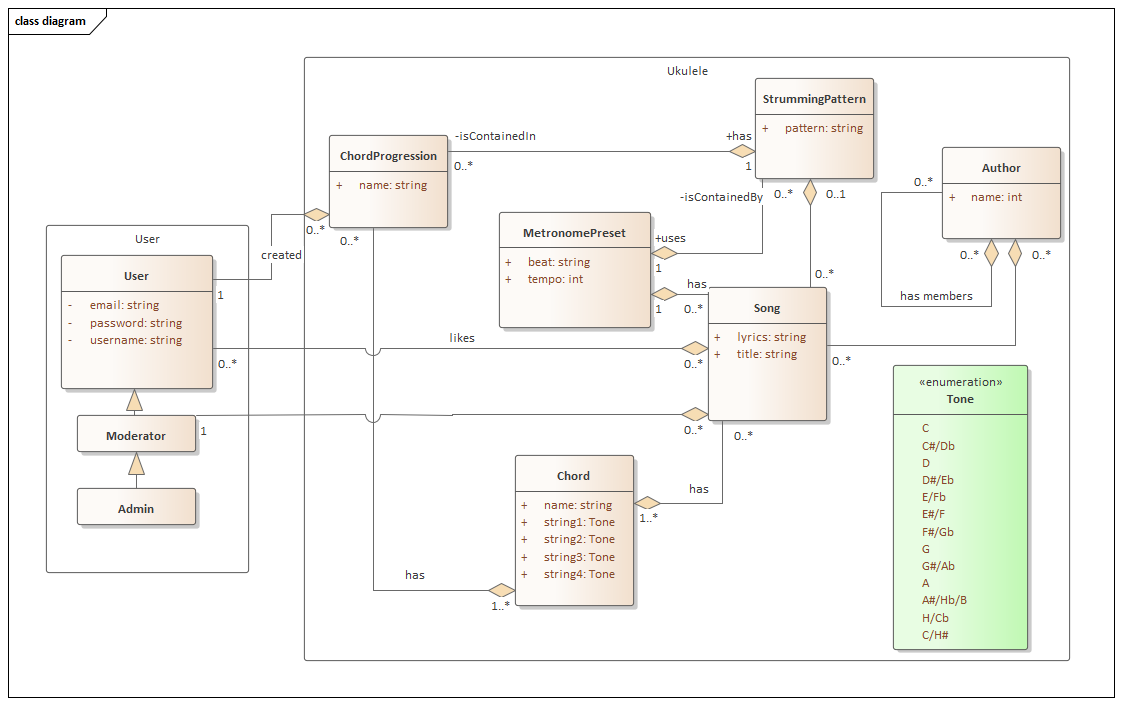
\includegraphics[width=\textwidth]{assets/class_diagram.png}
    \caption{Diagram tříd znázorňující domény}
    \label{fig:class_diagram}
\end{figure}

Backend část specifikuje veškerou práci s~daty, která se odehrává na serveru, od validace až po vystavování mutací a query pro GraphQL server. Tato část smí být závislá jen na společné části domény a modulu autorizace. Díky tomu se zajistí striktní oddělení domén a zjednoduší testování, jelikož jednotkové testy pak testují jen skutečně jednu funkcionalitu nezávisle na všech ostatních. Každý takovýto balíček exportuje jednu funkci, která jako parametr dostane nastavení a vrací objekt obsahující \emph{seed} pro inicializaci aplikace, mutace a query pro GraphQL server.

V~části frontend jsou vytvořeny jednotlivé komponenty, zase pouze pro jednu danou doménu. Tato část je závislá pouze na společné části domény, na modulu autorizace a na modulu \emph{look}, který udává vzhled aplikaci, tím že obsahuje základní komponenty, jako například tlačítko nebo základní vstupní pole. Takovýto balíček exportuje dané komponenty.

Takto rozdělené části tvoří balíčky. Tyto balíčky na sobě závisí, tak jak bylo popsáno výše a tyto závislosti jsou spravovány právě pomocí~\ref{ss:yarn} jako monorepo. Jednotlivé balíčky mají unifikované jména, a to takto:~\sloppy{\emph{uls@<doména>-<react|nodejs|common>}} kde uls je zkratka pro \emph{ukulele learning site}, což je pracovní název aplikace.

Jednotlivé balíčky ovšem netvoří výslednou aplikaci, proto je potřeba mít ještě další dva speciální balíčky, jeden pro backend a druhý pro frontend. Backend balíček importuje všechny inicializační funkce, vytvoří inicializační parametry, vytvoří jednotlivé moduly a následně je registruje do GraphQL serveru. Frontend balíček nejen, že importuje všechny komponenty, ale následně je skládá na stránky. Jednotlivé komponenty tedy neví, v~jakém kontextu a kde budou zobrazeny, a proto je potřeba aby byly správně zapouzdřené a komunikovali jen pomocí vstupních parametrů. Top level balíček, který je nadřazený všem, vytváří pouze testovací prostředí a slouží jako root balíček pro všechny moduly tak, aby mohlo správně fungovat monorepo.


\begin{figure}
    \dirtree{%
        .1 root projektu.
        .2 modules\DTcomment{Adresář s~moduly}.
        .3 look\DTcomment{Modul udávající vzhled aplikace}.
        .4 react.
        .3 ukulele\DTcomment{Modul obsahující doménu hry na ukulele}.
        .4 common.
        .4 nodejs.
        .4 react.
        .3 \ldots .
        .2 packages.
        .3 nodejs\DTcomment{Sestavuje backend server}.
        .3 react\DTcomment{Sestavuje frontend server}.
    }
    \caption{Zjednodušená adresářová struktura}
    \label{fig:modules}
\end{figure}

\subsection{Clean Architecture}
\label{ss:clean_architecture}
Tato metodika, prezentovaná ve stejnojmenné knize od R. C. Martina~\cite{martin_2018_clean}, popisuje jak rozdělit aplikaci na jednotlivé vrstvy. Říká, že aplikace by měla být rozdělena na \emph{entity}, \emph{use case}, \emph{presenters, controllers} a \emph{frameworks, drivers}, znázorňující obrázek~\ref{fig:clean_architecture}.
Entity definují základní byznys pravidla dané domény a jejich reprezentace může být například sada funkcí, nebo objekt s~metodami nebo bez. V~rámci této práce jsou entity reprezentovány pomocí objektů bez metod, přesněji TypeScript interfaces, a to hlavně z~důvodu snadné serializace a deserializace.
Vrstva use case provadí operace specifické pro aplikaci nad danými entitami. V~případě této práce to jsou \emph{intereactory}, třídy které manipulují s~entitami.
Následující vrstva už převádí dané entity na objekty vhodné pro další vrstvu frameworků, jedná se tedy o~interface. V~této práci je tato vrstva Mongoose modely, se kterými následně pracuje databáze a zároveň ze kterých se generuje GraphQL API, kterým backend předává informace frontendu. A~poslední vrstvou jsou samotné frameworky či databáze, v~případě této práce se jedná o~React, resp. MongoDB, které informace zobrazují, resp. ukládají.

Výhodou tohoto rozdělení je přehlednost a snadné testování. Při testování dané vrstvy, se vždy přistupuje z~vrstvy nadřazené, test tedy simuluje operace, které by dělala vrstva nadřazená a mockuje se první podřazená vrstva. Je tedy vždy jasné, jak daný test funguje a jaká data testuje. V~případe těchto testů mluvíme o~testech jednotkových, nikoliv smoke nebo integračních.

\begin{figure}
    \centering
    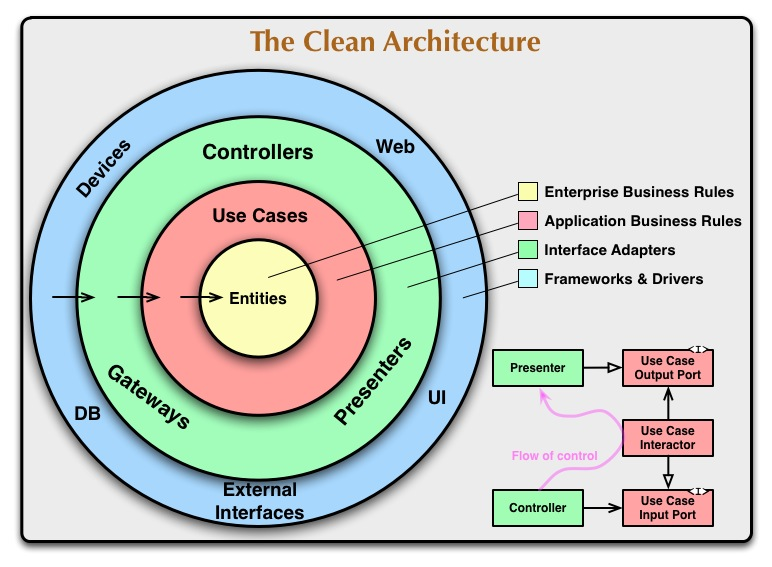
\includegraphics[width=\textwidth]{assets/clean_architecture.jpg}
    \caption{Clean Architecture \cite{martin_2019_clean}}
    \label{fig:clean_architecture}
\end{figure}



\section{Frontend}
\label{sc:frontend}

\subsection{Local state managment}
\label{ss:local_state_management}

\subsection{SSR}
\label{ss:ssr}

\subsection{Themes}
\label{ss:themes}

\section{Backend}
\label{sc:backend}

\subsection{Generování API}
\label{ss:api_generating}



\chapter{Testování}
\label{ch:testing}
Je několik různých typů testů, které se navzájem doplňují nebo překrývají. V rámci této práce byly vytvořeny automatické testy jednotkové a integrační a to za pomoci nástroje \nameref{ss:jest}. V následujících sekcích se podíváme právě na jednotkové a integrační testy, na další možnosti testování a na finální zhodnocení aplikace a budoucí vývoj.

\section{Jednotkové testy}
\label{sc:unit_tests}
Jednotkový test je typ testu, který testuje jednotlivé třídy, metody a funkce nezávisle na zbytku aplikace. Jak již bylo zmíněno v sekci \nameref{ss:clean_architecture}, rozdělení na vrstvy ulehčí testování. V rámci práce jsou takto testovány intereactory, které provádí změny nad entitami. Tím je zajištěno že všechny operace s entitami a to jak na backendu, tak na frontendu jsou validní.

\section{Integrační testy}
\label{sc:unit_tests}
Na rozdíl od jednotkového testu, který testuje jednotlivé nezávislé funkce čí metody, tak test integrační testuje více částí aplikace najednou. Zjistí se tím funkčnost celého systému. Bohužel, kvůli volbě verzi \nameref{ss:yarn} nebylo možné správně nakofigurovat řádný integrační test. První pokus bylo rozšíření pro \nameref{ss:storybook} \emph{storyshots}, který při spuštění vytvoří obrázky daných komponent a při dalších spuštěních je srovnává s předchozí verzí a případně notifikuje vývojáře. Další pokus byla konfigurace knihovny \emph{Cypress}, která umožňuje vytvářet \acrfull{e2e} testovací scénáře, které simulují průchody aplikací. Oba pokusy selhaly kvůli špatné integraci knihovny \emph{babel}, která transpiluje typescriptové soubory na soubory javascriptové a vytváří cesty k externím knihovnám, což byl práě důvod neúspěchu.

\section{Ostatní testy}
Samozřejmě existuje více druhů testů než pouze \hyperref[sc:unit_tests]{jednotkové} a \hyperref[sc:unit_tests]{integrační}. V rámci této práce by nás mohli zajímat hlavně testy akceptační a smoke. Akceptační test je v pravém slova smysl test klientem kterému předáváme software. V rámci této práce by se za akceptační test dal považovat test uživateli, který ale nemohl být uskutečněn a to kvůli absenci dat. Smoke testy jsou testy nasazení. Po nasazení se spustí jednoduchá testovací sada, která má za úkol ověřit zdali se aplikace správně nasadila a odpovídá.

\section{Budoucí vývoj}
\label{sc:upcomming_development}
Aplikace je nyní ve fázi funkčního prototypu, jsou implementovány všechny základní požadavky, ale stále je zde prostor na zlepšení. V následujících sekcích jsou rozebrány některé takové faktory.

\subsection{Doprání testů}
Asi největším nedostatkem aplikace je absence \hyperref[sc:unit_tests]{integračních testů}, což koncového uživatele může, ale nemusí postihnout. Tento nedostatek půjde vyřešit ve chvíli, kdy vývojáři babelu plně dokončí integraci nové verze yarnu. Do té doby bohužel není možnost takové testy psát, protože všechny testovací frameworky, které umožňují více než jen jednotkové testy, na této knihovně závisí.

\subsection{Data}
To co nejvíce aplikaci schází v tuto dobu jsou funkční data. Tím jsou myšleny písně s texty, akordy atd. Tyto data se dají jednoduše najít, ale pro osobní použití. Bohužel není žádné API poskytující seznam písní s textem a akordy pro ukulele. Tato data by se dala získat buď přepisem z jiných stránek či jejich scrapovaním, což by už mělo přesah do autorského zákona. Další možnost je kontaktovat přímo vydavatele a uzavřít spolupráci, která avšak nejspíš bude velmi finančně náročná. Poslední možnost by byla uzavřít spolupráci s již existujícímí aplikacemi a získat data od nich.

\subsection{Úpravy aplikace}
Hlavním neduhem stávající aplikace je hlavně design. Aplikace je sice ve dvou barevných schématech, ty však nejsou zcela vyladěné. Samotná úprava barev a rozložení nebude náročná, díky dělení na komponenty a použití globálně dostupných barevných schémat. Zároveň je možné v budoucnu přidat další barevná schémata na vrch dvou stávajících.

\subsection{Překlad}
Důležitou součástí aplikace, která míří na mezinárodní trh, tak je co největší jazyková dostupnost. Další krokem úpravy aplikace by tedy mělo být překlad do dalších jazyků, pro přilákání co největší skupiny uživatelů.

\subsection*{Podpora vybrnkávání}
Vybrnkávání je styl hraní na ukulele, kde se nehraje přejíždněním přes všechny struny, ale o některé se brnká. Tento styl má uplně jiný styl zobrazení. Jsou zobrazeny jednotlivé struny a k nim čísla pražců. Tato čísla jsou rozdělena do sloupců, které odpovídají době. Příklad takové tablatury je na obrázku \ref{fig:tablature}

\begin{figure}[h!]
    \centering
    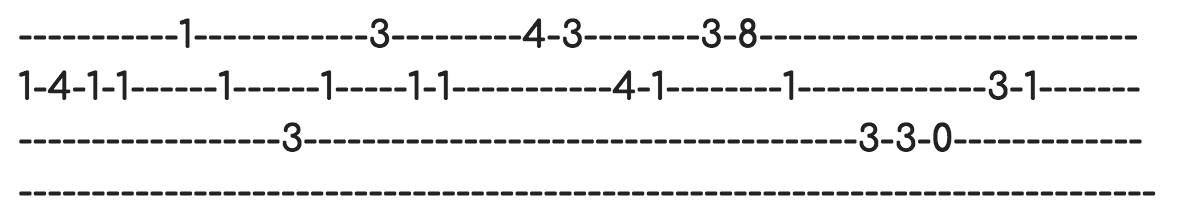
\includegraphics[width=\textwidth]{assets/picking.png}
    \caption{Noty pro vybrnkávání}
    \label{fig:tablature}
\end{figure}

\subsection*{Nastavení ladění}
Tato funkcionalita je témeř imlementována. Komponenta vykreslovaného akordu dostává na vstupu mimo akordu k vykreslení i aktuální ladění, které je vždy nastaveno na \emph{gcea}. Rozšíření by tedy spočívalo v přidání možnosti uživateli si toto ladění změnit, případně uložit pro příští návštěvy.



\chapter{Kontinuální integrace a nasazení}
\label{ch:ci_cd}
Kontinuální integrace, dodání a nasazení jsou přístupy k~automatizaci jednotlivých procesů, které jsou mezi vývojem a nasazením aplikace. V~rámci této práce si pouze nastíníme, co jednotlivé výrazy znamenají.

Kontinuální integrace se zabývá automatickou validací kódu pomocí automatizovaných testů. Tyto testy jsou spuštěny ve chvíli kdy programátor nahraje do systému správy verzí (\acrshort{scm}). Tyto automatické testy ověří funkčnost, správnost a další požadavky na aplikaci a následně zpětně informují vývojáře, resp. tým o~výsledcích testů. V~praxi se to běžně využívá před zapojením nové části kódu do celé aplikace. Výhodou tohoto přístupu je minimalizování chyb a zvýšení produktivity programátora. V~této práci kontinuální integrace byla realizována pomocí \emph{GitHub Actions}. Jelikož je celá aplikace open source a uložena na serveru \href{www.github.com}{github.com}, tak má nárok na využití systému GitHub Actions, který právě umožňuje automatické spouštění testů. Konkrétní testy prováděné automaticky jsou~\hyperref[sc:unit_tests]{jednotkové} a následně smoke build storybooku, který pouze ověří, zdali lze sestavit, tedy zdali aplikace lze sestavit. \cite[s.~7]{rossel_2017_continuous}

Kontinuální dodání a nasazení jsou pojmy velmi podobné. Kontinuální dodání vytvoří balíčky aplikace připravené k~nasazení a kontinuální nasazení je rovnou i nasadí. Jak dodání, tak nasazení je spouštěno automaticky po úspěšném provedení kontinuální integrace, nebo jiných krocích. V~praxi to může být manuální spuštění na konci sprintu nebo automaticky po zařazení kódu do hlavní větve. \cite[s.~18]{rossel_2017_continuous} Při tvorbě této aplikace bylo využito obojího. Při každé změně k~hlavní větvi jsou spuštěny dva nasazovací skripty. První zajišťuje automatické sestavení dokumentace a statické verze storybooku a nasazení na \emph{GitHub Pages}. Tato dokumentace je veřejně dostupná a hostovaná na serveru GitHub\footnote{\href{https://danbalarin.github.io/ukulele-learning-site/}{danbalarin.github.io/ukulele-learning-site/}}. Druhý sestavuje výslednou aplikaci, vytváří docker kontejnery a následně spustí aktualizaci na vzdáleném serveru. Docker kontejnery jsou vytvořeny dva, jeden pro backend a druhý pro frontend a jsou uloženy na veřejném docker repozitáři\footnote{\href{https://hub.docker.com/repository/docker/kenny11/uls-react}{hub.docker.com/repository/docker/kenny11/uls-react}}\footnote{\href{https://hub.docker.com/repository/docker/kenny11/uls-nodejs}{hub.docker.com/repository/docker/kenny11/uls-nodejs}}. Následně se skript připojí přes ssh k~vzdálenému serveru, spustí jednoduchý skript, který zastaví běžící instance, smaže, nahraje nové a spustí je. Jako poslední krok je spuštěn jednoduchý smoke test~\ref{code:smoke}, který ověří, zdali frontend odpovídá na portu 80, a backend odpovídá na portu 4000.

\begin{figure}[h!]
    \centering
    \begin{minted}{bash}
curl -sSL --max-time 5 -D - $URL:$PORT -o /dev/null
    \end{minted}
    \caption{Smoke test ověřující funkčnost http serveru}
    \label{code:smoke}
\end{figure}


\begin{conclusion}
    Cílem práce bylo vytvořit aplikaci pro podporu výuky hry na ukulele v~souladu s~metodami softwarového inženýrství. Ve zkratce jsem uvedl, co je potřeba znát pro hraní na ukulele. Prozkoumal jsem již existující aplikace a zvážil jejich výhody a nevýhody. Dále jsem uvedl dostupné technologie a cílovou skupinu, pro kterou je aplikace tvořena. Na základě těchto poznatků jsem stanovil funkční a nefunkční požadavky, ze kterých jsem vytvořil případy užití, wireframy a diagram tříd. Následně jsem zvolil technologie, které jsem využil k~vytvoření aplikace. Popsal jsem metodiky použité k~návrhu architektury aplikace a určil logické členění částí aplikace. Na základě návrhu jsem implementoval prototyp aplikace a automatické testy aplikace. Poté jsem vytvořil testovací a nasazovací skripty, které pracují zcela automaticky.

    Prototyp aplikace je plně funkční, umožňuje vyhledávat akordy, strumming patterny, písně i autory. Uživatel má možnost se přihlásit a tím zpřístupnit nastavování písní jako oblíbené. Moderátor může přidávat, či upravovat písně a autory a administrátor může měnit role vytvořených účtů. Aplikace je dostupná v~anglickém jazyce.

    Aplikaci lze rozšířit o~další funkcionality, třeba vybrnkávání, či nastavování vlastního ladění ukulele. Vhodné by bylo aplikaci rozšířit o~další jazyky či vylepšit grafické pojetí. Dobrým nápadem je z~responzivní aplikace udělat \hyperref[sss:pwa]{progresivní webovou aplikaci}.

    Hlavní přínos práce spočívá v~přehlednosti a jednoduchosti aplikace, z~čehož benefitují hlavně uživatelé méně zkušení s~počítačem. Zvolené technologie umožnily rychle a efektivně vytvořit aplikaci, kterou je možné jednoduše rozšířit, či upravit. Jediná nevýhoda zvolených technologií je špatná kompatibilita, což znemožnilo integrační testování. Tento problém by však měl v~budoucnu s~rostoucí komunitou vymizet a aplikaci tedy bude možné o~dané testy rozšířit a tím zajistit konzistenci kvality.
\end{conclusion}

\printbibliography[title={Literatura}]

\appendix

\chapter{Seznam použitých zkratek}
% \printglossaries
\begin{description}
	\item[GUI] Graphical user interface
	\item[XML] Extensible markup language
\end{description}

\chapter{Obsah přiloženého CD}

%upravte podle skutecnosti

\begin{figure}
	\dirtree{%
		.1 readme.txt\DTcomment{stručný popis obsahu CD}.
		.1 build\DTcomment{adresář se spustitelnou formou implementace}.
		.2 react\DTcomment{adresář se spustitelným frontend serverem}.
		.2 nodejs\DTcomment{adresář se spustitelným backend serverem}.
		.1 src.
		.2 impl\DTcomment{zdrojové kódy implementace}.
		.2 thesis\DTcomment{zdrojová forma práce ve formátu \LaTeX{}}.
		.2 thesis.pdf\DTcomment{text práce ve formátu PDF}.
	}
\end{figure}

\end{document}
